\subsection{Churn Aware Resource Allocation}

\subsubsection{Churner Classification}
Naive Bayesian Classifier is chosen because it is computationally efficient and degree of churn is equal to the posterior probability, however, other approaches, such as regression, decision trees, neural networks etc. can also be used. Machine learning framework using Naive Bayesian classifier is shown in Figure~\ref{classification}.
\begin{figure}[!h]
\centering
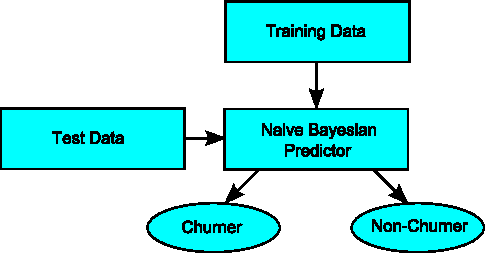
\includegraphics[width=3.5in]{pic/classification.pdf}
\caption{Machine learning framework for churner classification using Naive Bayes classifier}
\label{classification}
\end{figure}

\begin{table}[!h]
\caption{Cloud Customer Data (inspired by Telecom user dataset)}
\label{table1}
\centering
\begin{tabular}{|p{1.1cm}|p{3cm}|p{3cm}|}
\hline
\hline
Data type&Description&Example\\
\hline
\hline
number&customer ID&019164958, 019164958..\\
\hline
date&Date of birth&19610425, 19440112...\\
\hline
number&zip code&08648, 20774...\\
\hline
int&bills of customers&15219, 15249...\\
\hline
int&service plan&1, 2, 3, 4\\
\hline
int&total duration of service&57, 21...\\
\hline
int&churner or non-churner&0, 1\\
\hline
\end{tabular}
\end{table}
Attributes associated with customers of cloud service providers may look like as shown in Table~\ref{table1}. Customer data is treated as vectors denoted as $X=\{x_1,x_2,...,x_n\}$  with $n$ attributes. Naive Bayesian Predictor is trained by feeding the vectors X and labels. The trained predictor maps vectors $X_i$ to label $Y_j$ for every $i^{th}$ feature in customer data and for every class $j$. And then we compute probability $P(X_i,i\in n|Y_j, j\in m)$, which contain n features and m classes, in this case m has two values that are 1 and 0 representing classes $churn$ and $non-churn$ respectively. According to Bayes' theorem:
\begin{equation*}
P(Y)P(X|Y)=P(X)P(Y|X)
\end{equation*}
$P(X|Y)$ donate to probability of each feature given class $Y$,and $P(Y|X)$ is the probability of each class given feature $X$. The class for which we get maximum value $\sum_{i=1}^n P(Y_j|X_i)$ the customer belongs to that class. In the case of two classes, $churn$ and $non-churn$,  if the probability of $churn$ is higher than probability of $nonchurn$, then the customer belongs to the class $churn$. Furthermore, if a customer belongs to class $churn$ then the degree of churn is computed as below,
\begin{equation}
D_i=\sum_{i=1}^n P(Class=churn|X_i) 
\label{eq:degchurn}
\end{equation}

\subsubsection{Resources Allocation}
Cloud users pay for cloud resources according to equation~\ref{eq:reveneue}. If a user is identified as churner, retention action according to equation~\ref{fixed} is computed. Moreover, to improve churner satisfaction level, additional resources is given according to retention strategy as described in last section. The churner will get an added capacity, therefore, final capacity for some churner $i$ is computed as below:
\begin{equation*}
O_{i}=\dfrac{p_{i}+RC_{i}-\beta}{\alpha}
\end{equation*}

\subsection{Virtual Machine Placement}
 Virtual machines characterized by allocated resources are placed on physical machines. In our work, we assume that one PM can host multiple VMs. For demonstration purposes, we assume a single VM represents a single user. It is to be noted that our work can be easily expanded to multiple VM request per user.
\subsubsection{Linear Programming Formulation}
Every physical machine $j$ is characterized by 2-tuple, $\{Q_j,C_j\}$ where $Q_j$ and $C_j$ are capacity and costs associated with a physical machine respectively. Virtual machine placement problem is formulated as linear programming problem for profit maximization as below: \\


$Maximize:$
\begin{equation}
\label{Pro}{(\sum_{i=1}^n (\alpha O_i+\beta))-\sum_{j\in TO} C_j }
\end{equation}

$Constraints:$
\begin{equation}
\label{Con1}
\sum_{i=1}^n\theta_{ij}=1 \forall j
\end{equation}

\begin{equation}
\label{Con2}
Q_j\geqslant \sum_{i=1}^n\theta_{ij} O_i+H_j
\end{equation}

The first part in equation~\ref{Pro} is revenue and the second part is cost of runningm physical machine. Since there is flat cost associated with each physical machines, our profit maximization problem becomes cost minimization problem. 
The first constraint states that one VM is allocated to one PM (equation~\ref{Con1}). Second constraint (equation \ref{Con2}) states that capacity of VMs and overhead should not exceed the total capacity of a PM (refer equation~\ref{totaloverhead} for $H_j$). 


%In this bar chart, the PPR decreases from left to right. So that mean the more PMs close to left turns on the less money will be cost. For determining which PMs need to be turned on, there are two algorithms which are First-Fit and Best-Fit.

%\subsection{Placement Algorithm 1}
%Since cloud provider got the capacity of each VM, and capacity of PMs are also known, so it just puts VMs into these PMs based on the rank. In this case, the PM10 (35GHz, 20\$) will be used first. From left to right, so the next is PM8, then PM9, so on and so force. Till all VMs are placed on PMs, then cloud provider will know which PMs need to be turned on.
%\begin{algorithm}
 %\caption{Placement Algorithm 1}
 %\begin{algorithmic}[1]
 %\renewcommand{\algorithmicrequire}{\textbf{Input:}}
 %\renewcommand{\algorithmicensure}{\textbf{Output:}}
 %\REQUIRE Physical machines(PM) with {cost of running each PM, number of cores, and core frequency(GHz)}, virtual machines(VM)
 %\ENSURE  running Physical machines, and total cost of running Physical machines
 %\STATE calculate the cost performance of PMs
 %\STATE rank PMs according to cost performance
 %\\ \textit{LOOP Process}
  %\FOR {each VM i}
  %\FOR {each PM j}
  %\STATE check if there is a core in the CPU can process the VM
  %\STATE occupy = Occupied\_PM(j)+VM(i)+overhead
  %\IF {occupy<PM(i)}
  %\STATE assign the VMi to the PMj
  %\ENDIF
  %\ENDFOR
  %\ENDFOR
  %\STATE compute the cost of running physical machine
 %\end{algorithmic} 
 %\end{algorithm}
 
\subsubsection{Best Fit Heuristics}

  \begin{algorithm}
 \caption{VM Placement Algorithm}
 \begin{algorithmic}[1]
 \renewcommand{\algorithmicrequire}{\textbf{Input:}}
 \renewcommand{\algorithmicensure}{\textbf{Output:}}
 \REQUIRE Physical Machines (PMs) with {cost of PMs, number of cores, and core frequency (GHz)}, Virtual Machines (VMs)
 \ENSURE  Virtual Machines assignment to Physical machines, and profit
 \STATE calculate the cost - performance ratio of PMs
 \STATE rank PMs according to cost - performance ratio
 \\ \textit{LOOP Process}
  \FOR {each $PM_j$}
  \STATE check if there is a core that can process VMs
  \STATE check occupied size of $PM_j$
  \FOR{each $VM_i$}
  \STATE find the maximal $VM_i$ that can be assigned to $PM_j$
  \STATE occupy = Occupied\_$PM_j$+$VM_i$+overhead
  \IF {occupy$< PM_j$}
  \STATE assign the $VM_i$ to the $PM_j$
  \ENDIF
  \ENDFOR
  \ENDFOR
  \STATE compute the Profit 
  \STATE return profit, run PMs
 \end{algorithmic} 
 \end{algorithm}
%For a single PM, it can be used for multiple VMs. Actually we are going to divide a PM into many VMs, the physical resources support multiple VMs. However, we can abstract this problem to a Bin Packing algorithm by an opposite strategy. Totally, a PM has certain physical resources which VMs are not. VM resources are various due to the different requirements from customers, and VMs use the certain physical resources form PMs. Based on these theories, we assume PMs are bags, and VMs are the things need to be putted into these bags. Obviously, each VM has different capacity that meaning they have diverse weights. Meanwhile, PMs also have different capacities and costs. We have mentioned above, to minimize summarized cost is equal to maximize profit because of the revenue is fixed. So to reduce the cost is to use less physical machines. But here is an issue that how do cloud provider decided to turn on which physical machines?
The optimization problem described in the last section is NP complete. In this section, we suggest a heuristics to solve this problem in linear time. Note that physical machines can be distinguished by only this 2-tuple-(${Q_j,C_j}$).  Algorithm 1 describes the solution for VM placement problem. PMs are sorted in decreasing order of performance/price ratio (PPR) given by $\frac{Q_j}{C_j}$. Then we apply best-fit heuristics to solve the linear programming problem presented in last subsection.

%Another placement strategy is called Best-Fit Algorithm, compared with First-Fit Algorithm, this one has an obvious advantage that every used core is as full as possible, system always seek the most suitable VM to place on the current core so that each core has a high-usage. If we do this way, the disadvantage point is we need to set up a monitor program to listen all current VMs and traverse all VMs to find the most suitable one, assuredly, this way may raise the manager node workload.
